\section{Technical information gathering}

\subsection{Spacex (30p)}
\addtocounter{points}{30}

Can you find the main SpaceX - Starlink ipv4 network range? Write it in CIDR format!

\textbf{Solution:}\\
For this task I looked up \url{starlink.com} on dnsdumpster and found an ip hosted from SpaceX - Starlink.

\begin{center}
    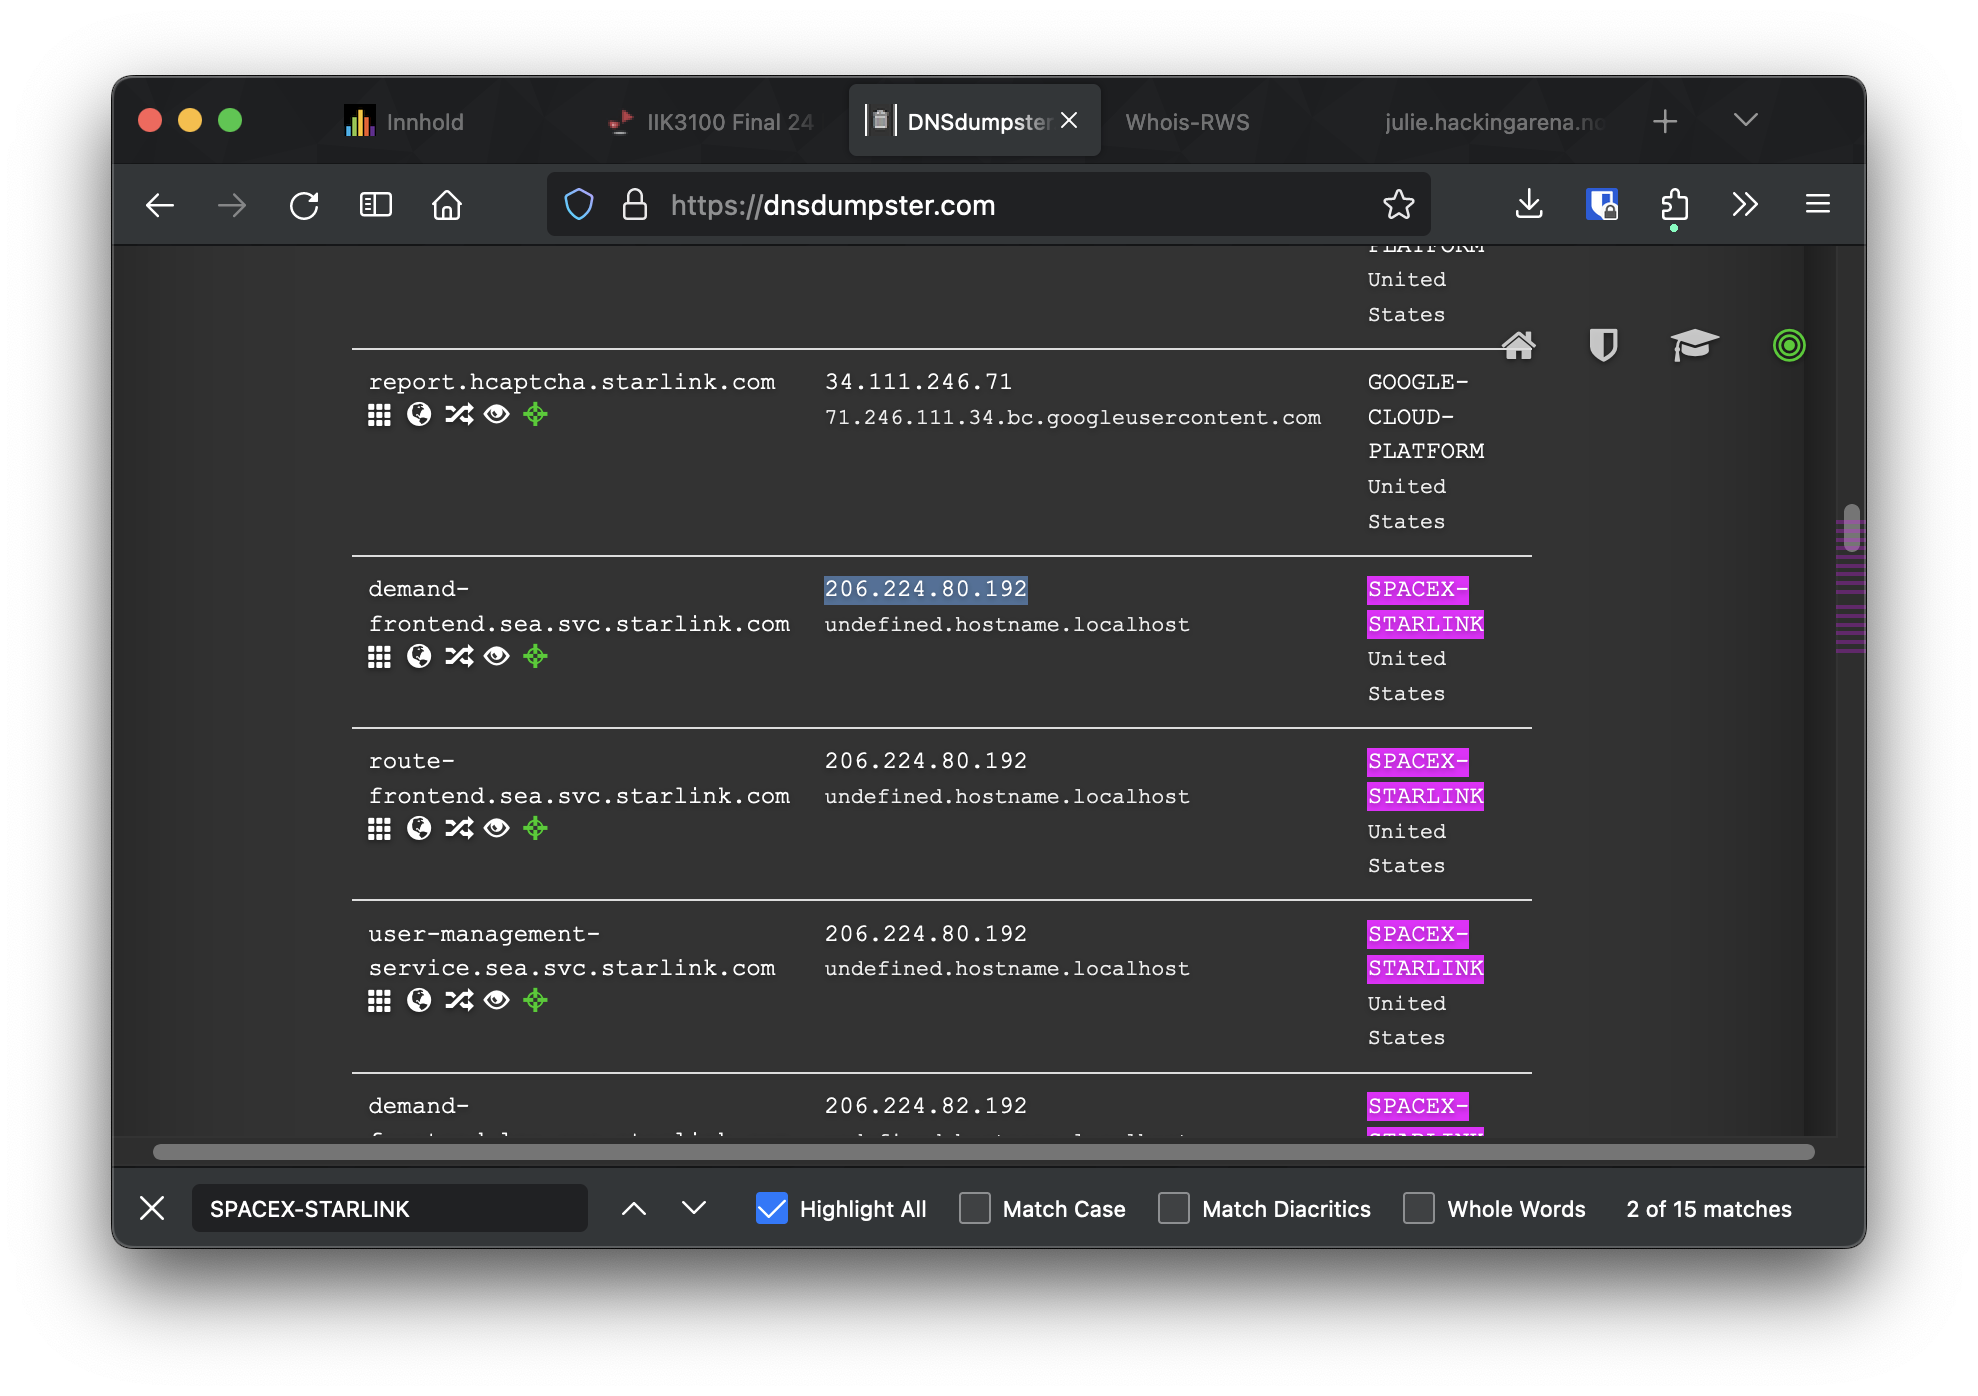
\includegraphics[width=12cm]{img/Technical information gathering/Spacex/Screenshot 2023-11-24 at 11.01.46.png}
\end{center}

After finding the ip I looked it up on ARIN and found the network range:

\begin{center}
    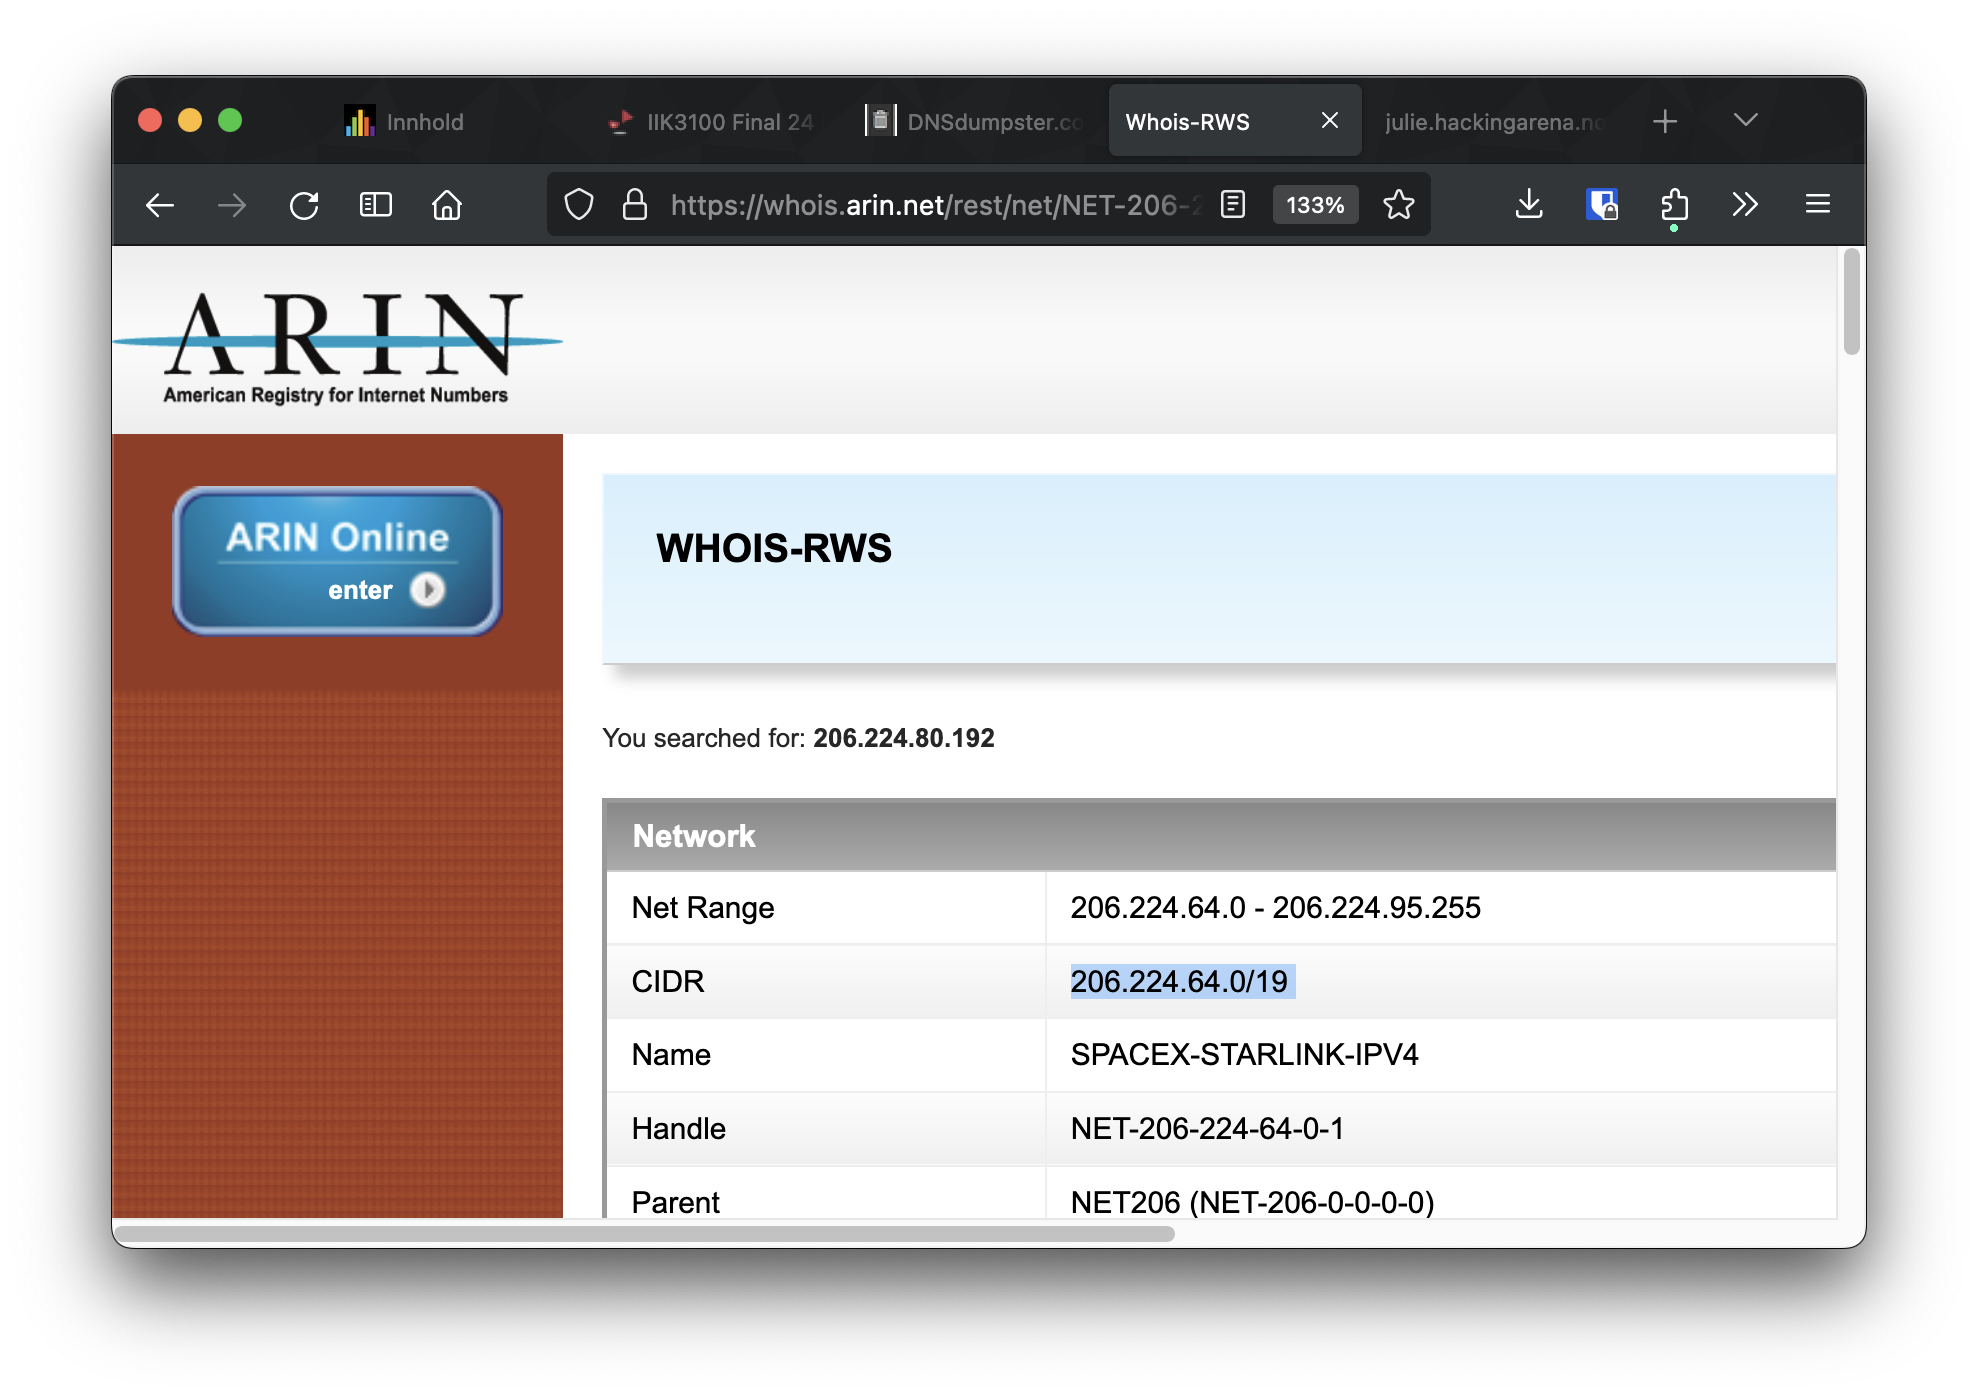
\includegraphics[width=11cm]{img/Technical information gathering/Spacex/Screenshot 2023-11-24 at 11.02.02.png}
\end{center}

\newpage
\subsection{Mysql in Lillesand (30p)}
\addtocounter{points}{30}
There are 3 mysql services available in Lillesand, can you find the ip of one of them?

Don't portscan anyone! Use only open source tools!

\textbf{Solution:}\\
For this task I used \url{search.censys.io} to search for mysql services located in Lillesand.

\begin{center}
    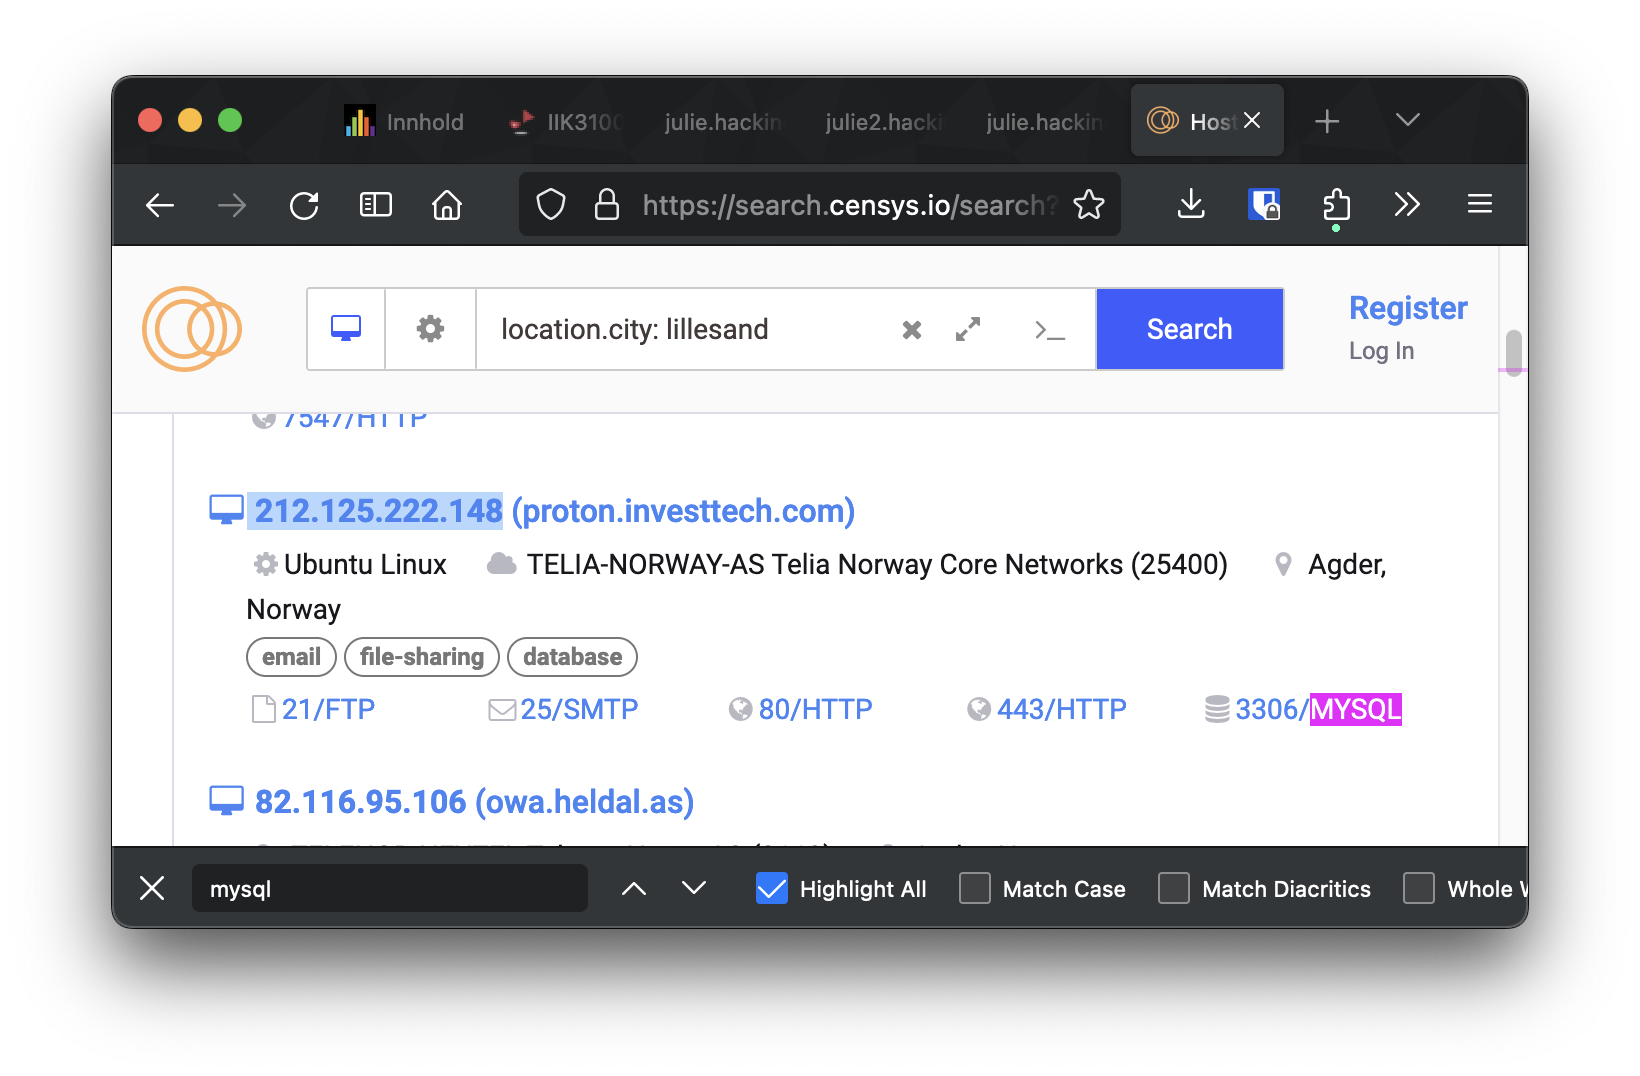
\includegraphics[width=15cm]{img/Technical information gathering/Mysql Lillesand/Screenshot 2023-11-24 at 11.16.26.png}
\end{center}